%==============================================================================
% Tento soubor použijte jako základ
% This file should be used as a base for the thesis
% Autoři / Authors: 2008 Michal Bidlo, 2022 Jaroslav Dytrych
% Kontakt pro dotazy a připomínky: sablona@fit.vutbr.cz
% Contact for questions and comments: sablona@fit.vutbr.cz
%==============================================================================
% kódování: UTF-8 (zmena prikazem iconv, recode nebo cstocs)
% encoding: UTF-8 (you can change it by command iconv, recode or cstocs)
%------------------------------------------------------------------------------
% zpracování / processing: make, make pdf, make clean
%==============================================================================
% Soubory, které je nutné upravit nebo smazat: / Files which have to be edited or deleted:
%   projekt-20-literatura-bibliography.bib - literatura / bibliography
%   projekt-01-kapitoly-chapters.tex - Table des matières práce / the thesis content
%   projekt-01-kapitoly-chapters-en.tex - Table des matières práce v angličtině / the thesis content in English
%   projekt-30-prilohy-appendices.tex - přílohy / appendices
%   projekt-30-prilohy-appendices-en.tex - přílohy v angličtině / appendices in English
%==============================================================================
\documentclass[]{fitthesis} % bez zadání - pro začátek práce, aby nebyl problém s překladem
%\documentclass[english]{fitthesis} % without assignment - for the work start to avoid compilation problem
%\documentclass[zadani]{fitthesis} % odevzdani do IS VUT a/nebo tisk s barevnými odkazy - odkazy jsou barevné
%\documentclass[english,zadani]{fitthesis} % for submission to the IS VUT and/or print with color links - links are color
%\documentclass[zadani,print]{fitthesis} % pro černobílý tisk - odkazy jsou černé
%\documentclass[english,zadani,print]{fitthesis} % for the black and white print - links are black
%\documentclass[zadani,cprint]{fitthesis} % pro barevný tisk - odkazy jsou černé, znak VUT barevný
%\documentclass[english,zadani,cprint]{fitthesis} % for the print - links are black, logo is color
% * Je-li práce psaná v anglickém jazyce, je zapotřebí u třídy použít 
%   parametr english následovně:
%   If thesis is written in English, it is necessary to use 
%   parameter english as follows:
%      \documentclass[english]{fitthesis}
% * Je-li práce psaná ve slovenském jazyce, je zapotřebí u třídy použít 
%   parametr slovak následovně:
%   If the work is written in the Slovak language, it is necessary 
%   to use parameter slovak as follows:
%      \documentclass[slovak]{fitthesis}
% * Je-li práce psaná v anglickém jazyce se slovenským abstraktem apod., 
%   je zapotřebí u třídy použít parametry english a enslovak následovně:
%   If the work is written in English with the Slovak abstract, etc., 
%   it is necessary to use parameters english and enslovak as follows:
%      \documentclass[english,enslovak]{fitthesis}

% Základní balíčky jsou dole v souboru šablony fitthesis.cls
% Basic packages are at the bottom of template file fitthesis.cls
% zde můžeme vložit vlastní balíčky / you can place own packages here


% Pro seznam zkratek lze využít balíček Glossaries - nutno odkomentovat i níže a při kompilaci z konzoly i v Makefile (plnou verzi pro Perl, nebo lite)
% The Glossaries package can be used for the list of abbreviations - it is necessary to uncomment also below. When compiling from the console also in the Makefile (full version for Perl or lite)
%\usepackage{glossaries}
%\usepackage{glossary-superragged}
%\makeglossaries 

% Nastavení cesty k obrázkům
% Setting of a path to the pictures
%\graphicspath{{obrazky-figures/}{./obrazky-figures/}}
%\graphicspath{{obrazky-figures/}{../obrazky-figures/}}

%---rm---------------
\renewcommand{\rmdefault}{lmr}%zavede Latin Modern Roman jako rm / set Latin Modern Roman as rm
%---sf---------------
\renewcommand{\sfdefault}{qhv}%zavede TeX Gyre Heros jako sf
%---tt------------
\renewcommand{\ttdefault}{lmtt}% zavede Latin Modern tt jako tt

% vypne funkci šablony, která automaticky nahrazuje uvozovky,
% aby nebyly prováděny nevhodné náhrady v popisech API apod.
% disables function of the template which replaces quotation marks
% to avoid unnecessary replacements in the API descriptions etc.
\csdoublequotesoff

\usepackage{url}

% =======================================================================
% balíček "hyperref" vytváří klikací odkazy v pdf, pokud tedy použijeme pdflatex
% problém je, že balíček hyperref musí být uveden jako poslední, takže nemůže
% být v šabloně
% "hyperref" package create clickable links in pdf if you are using pdflatex.
% Problem is that this package have to be introduced as the last one so it 
% can not be placed in the template file.
\ifWis
\ifx\pdfoutput\undefined % nejedeme pod pdflatexem / we are not using pdflatex
\else
  \usepackage{color}
  \usepackage[unicode,colorlinks,hyperindex,plainpages=false,pdftex]{hyperref}
  \definecolor{hrcolor-ref}{RGB}{223,52,30}
  \definecolor{hrcolor-cite}{HTML}{2F8F00}
  \definecolor{hrcolor-urls}{HTML}{092EAB}
  \hypersetup{
	linkcolor=hrcolor-ref,
	citecolor=hrcolor-cite,
	filecolor=magenta,
	urlcolor=hrcolor-urls
  }
  \def\pdfBorderAttrs{/Border [0 0 0] }  % bez okrajů kolem odkazů / without margins around links
  \pdfcompresslevel=9
\fi
\else % pro tisk budou odkazy, na které se dá klikat, černé / for the print clickable links will be black
\ifx\pdfoutput\undefined % nejedeme pod pdflatexem / we are not using pdflatex
\else
  \usepackage{color}
  \usepackage[unicode,colorlinks,hyperindex,plainpages=false,pdftex,urlcolor=black,linkcolor=black,citecolor=black]{hyperref}
  \definecolor{links}{rgb}{0,0,0}
  \definecolor{anchors}{rgb}{0,0,0}
  \def\AnchorColor{anchors}
  \def\LinkColor{links}
  \def\pdfBorderAttrs{/Border [0 0 0] } % bez okrajů kolem odkazů / without margins around links
  \pdfcompresslevel=9
\fi
\fi
% Řešení problému, kdy klikací odkazy na obrázky vedou za obrázek
% This solves the problems with links which leads after the picture
\usepackage[all]{hypcap}


% Informace o práci/projektu / Information about the thesis
%---------------------------------------------------------------------------
\projectinfo{
  %Prace / Thesis
  project={BP},            %typ práce BP/SP/DP/DR  / thesis type (SP = term project)
  year={2025},             % rok odevzdání / year of submission
  date=\today,             % datum odevzdání / submission date
  %Nazev prace / thesis title
  title.cs={À EPITA},  % název práce v češtině či slovenštině (dle zadání) / thesis title in czech language (according to assignment)
  title.en={Promo 2023-2028}, % název práce v angličtině / thesis title in english
  %title.length={14.5cm}, % nastavení délky bloku s titulkem pro úpravu zalomení řádku (lze definovat zde nebo níže) / setting the length of a block with a thesis title for adjusting a line break (can be defined here or below)
  %sectitle.length={14.5cm}, % nastavení délky bloku s druhým titulkem pro úpravu zalomení řádku (lze definovat zde nebo níže) / setting the length of a block with a second thesis title for adjusting a line break (can be defined here or below)
  %dectitle.length={14.5cm}, % nastavení délky bloku s titulkem nad prohlášením pro úpravu zalomení řádku (lze definovat zde nebo níže) / setting the length of a block with a thesis title above declaration for adjusting a line break (can be defined here or below)
  %Autor / Author
  author.name={Keany Vy Khun, Theo Brulier, Nathan Gillotin},   % jméno autora / author name
  author.surname={},   % příjmení autora / author surname 
  %author.title.p={Bc.}, % titul před jménem (nepovinné) / title before the name (optional)
  %author.title.a={Ph.D.}, % titul za jménem (nepovinné) / title after the name (optional)
  %Ustav / Department
  department={UPGM}, % doplňte příslušnou zkratku dle ústavu na zadání: UPSY/UIFS/UITS/UPGM / fill in appropriate abbreviation of the department according to assignment: UPSY/UIFS/UITS/UPGM
  % Školitel / supervisor
  supervisor.name={},   % jméno školitele / supervisor name 
  supervisor.surname={Příjmení},   % příjmení školitele / supervisor surname
  supervisor.title.p={prof. RNDr.},   %titul před jménem (nepovinné) / title before the name (optional)
  supervisor.title.a={Ph.D.},    %titul za jménem (nepovinné) / title after the name (optional)
  % Klíčová slova / keywords
  keywords.cs={}, % klíčová slova v českém či slovenském jazyce / keywords in czech or slovak language
  keywords.en={Filtre de Canny, Transformation de Hough, Masque gaussien, Gradient d'intensité, Suppression des non-maxima, Seuillage adaptatif, Filtre grayscale, Filtre médian, Filtre moyen, Bibliothèque SDL, Convolution, Détection des bords, Segmentation, Prétraitement d'image, Rotation d'image, Découpage d'image, Solveur de mots croisés, Réseau neuronal}, % klíčová slova v anglickém jazyce / keywords in english
  %keywords.en={Here, individual keywords separated by commas will be written in English.},
  % Abstrakt / Abstract
  abstract.cs={\\Le projet OCaligraph est un logiciel de reconnaissance optique de caractères (OCR) développé par des étudiants de deuxième année à l'EPITA. \\\\ Ce document présente l'état d'avancement du projet pour la première soutenance de novembre. \\\\ À ce stade, l'équipe a réussi à mettre en place plusieurs éléments clés, notamment un solveur pour identifier les mots dans la grille de mots croisés, le prétraitement des images à l'aide de divers filtres pour améliorer leur lisibilité, ainsi que le découpage des images pour extraire les éléments pertinents. \\\\ De plus, une fonction de rotation d'image a été intégrée pour garantir une orientation correcte de la grille. \\\\ Le rapport décrit les techniques utilisées, telles que le filtre de Canny et la transformation de Hough pour la détection des bords et des lignes, tout en abordant les défis rencontrés durant le développement. \\\\ Enfin, il souligne les objectifs futurs, notamment l'amélioration du prétraitement et l'optimisation des fonctions existantes, offrant ainsi un aperçu complet des avancées du projet, des aspects techniques et organisationnels de l'équipe.},
  %declaration={I hereby declare that this Bachelor's thesis was prepared as an original work by the author under the supervision of Mr. X
% The supplementary information was provided by Mr. Y
% I have listed all the literary sources, publications and other sources, which were used during the preparation of this thesis.},
  % Poděkování (nepovinné, nejlépe v jazyce práce; nechcete-li, zakomentujte pro skrytí nadpisu) / Acknowledgement (optional, ideally in the language of the thesis; comment out for hiding including heading) acknowledgment={V této sekci je možno uvést poděkování vedoucímu práce a těm, kteří poskytli odbornou pomo (externí zadavatel, konzultant apod.).},
  %acknowledgment={Here it is possible to express thanks to the supervisor and to the people which provided professional help
%(external submitter, consultant, etc.).},
  % Rozšířený abstrakt (cca 3 normostrany) - lze definovat zde nebo níže / Extended abstract (approximately 3 standard pages) - can be defined here or below
  %extendedabstract={Do tohoto odstavce bude zapsán rozšířený výtah (abstrakt) práce v českém (slovenském) jazyce.},
  %extabstract.odd={true}, % Začít rozšířený abstrakt na liché stránce? / Should extended abstract start on the odd page?
  %faculty={FIT}, % FIT/FEKT/FSI/FA/FCH/FP/FAST/FAVU/USI/DEF
  faculty.cs={Fakulta informačních technologií}, % Fakulta v češtině - pro využití této položky výše zvolte fakultu DEF / Faculty in Czech - for use of this entry select DEF above
  faculty.en={Faculty of Information Technology}, % Fakulta v angličtině - pro využití této položky výše zvolte fakultu DEF / Faculty in English - for use of this entry select DEF above
  department.cs={Ústav matematiky}, % Ústav v češtině - pro využití této položky výše zvolte ústav DEF nebo jej zakomentujte / Department in Czech - for use of this entry select DEF above or comment it out
  department.en={Institute of Mathematics} % Ústav v angličtině - pro využití této položky výše zvolte ústav DEF nebo jej zakomentujte / Department in English - for use of this entry select DEF above or comment it out
}

% Rozšířený abstrakt (cca 3 normostrany) - lze definovat zde nebo výše / Extended abstract (approximately 3 standard pages) - can be defined here or above
%\extendedabstract{Do tohoto odstavce bude zapsán výtah (abstrakt) práce v českém (slovenském) jazyce.}
% Začít rozšířený abstrakt na liché stránce? / Should extended abstract start on the odd page?
%\extabstractodd{true}

% nastavení délky bloku s titulkem pro úpravu zalomení řádku - lze definovat zde nebo výše / setting the length of a block with a thesis title for adjusting a line break - can be defined here or above
%\titlelength{14.5cm}
% nastavení délky bloku s druhým titulkem pro úpravu zalomení řádku - lze definovat zde nebo výše / setting the length of a block with a second thesis title for adjusting a line break - can be defined here or above
%\sectitlelength{14.5cm}
% nastavení délky bloku s titulkem nad prohlášením pro úpravu zalomení řádku - lze definovat zde nebo výše / setting the length of a block with a thesis title above declaration for adjusting a line break - can be defined here or above
%\dectitlelength{14.5cm}

% řeší první/poslední řádek odstavce na předchozí/následující stránce
% solves first/last row of the paragraph on the previous/next page
\clubpenalty=10000
\widowpenalty=10000

% checklist
\newlist{checklist}{itemize}{1}
\setlist[checklist]{label=$\square$}

% Kompilace po částech (rychlejší, ale v náhledu nemusí být vše aktuální)
% Compilation piecewise (faster, but not all parts in preview will be up-to-date)
% Další informace viz / For more information see https://www.overleaf.com/learn/latex/Multi-file_LaTeX_projects
% \usepackage{subfiles}

% Nechcete-li, aby se u oboustranného tisku roztahovaly mezery pro zaplnění stránky, odkomentujte následující řádek / If you do not want enlarged spacing for filling of the pages in case of duplex printing, uncomment the following line
% \raggedbottom

\begin{document}
  % Vysazeni titulnich stran / Typesetting of the title pages
  % ----------------------------------------------
  \maketitle
  % Table des matières
  % ----------------------------------------------
  \setlength{\parskip}{0pt}

  {\hypersetup{hidelinks}\tableofcontents}
  
  % Seznam obrazku a tabulek (pokud prace Table des matièresuje velke mnozstvi obrazku, tak se to hodi)
  % List of figures and list of tables (if the thesis contains a lot of pictures, it is good)
  \ifslovak
    \renewcommand\listfigurename{Zoznam obrázkov}
  \fi
  {\hypersetup{hidelinks}}
  
  \ifslovak
    \renewcommand\listtablename{Zoznam tabuliek}
  \fi
  % {\hypersetup{hidelinks}\listoftables}

  % Seznam zkratek / List of abbreviations
  %\ifczech
  %  \renewcommand*\glossaryname{Seznam zkratek}%
  %  \renewcommand*\entryname{Zkratka}
  %  \renewcommand*\descriptionname{Význam}
  %\fi
  %\ifslovak
  %  \renewcommand*\glossaryname{Zoznam skratiek}%
  %  \renewcommand*\entryname{Skratka}
  %  \renewcommand*\descriptionname{Význam}
  %\fi
  %\ifenglish
  %  \renewcommand*\glossaryname{List of abbreviations}%
  %  \renewcommand*\entryname{Abbreviation}
  %  \renewcommand*\descriptionname{Meaning}
  %\fi
  % Definice zkratek - z textu se odkazují např. \Gls{TF–IDF}
  % Definition of abbreviations - referred from the text e.g. \Gls{TF–IDF}
  %\newglossaryentry{TF–IDF}
  %{
  %  name={TF–IDF},
  %  description={Term Frequency-Inverse Document Frequency}
  %}
  % 
  %\setglossarystyle{superragged}
  %\printglossaries


  \ifODSAZ
    \setlength{\parskip}{0.5\bigskipamount}
  \else
    \setlength{\parskip}{0pt}
  \fi

  % vynechani stranky v oboustrannem rezimu
  % Skip the page in the two-sided mode
  \iftwoside
    \cleardoublepage
  \fi

  % Text prace / Thesis text
  % ----------------------------------------------
  \ifenglish
    \input{projekt-01-kapitoly-chapters-en}
  \else
    % Tento soubor nahraďte vlastním souborem s Table des matièresem práce.
%=========================================================================
% Autoři: Michal Bidlo, Bohuslav Křena, Jaroslav Dytrych, Petr Veigend a Adam Herout 2019

% Pro kompilaci po částech (viz projekt.tex), nutno odkomentovat a upravit
%\documentclass[../projekt.tex]{subfiles}
%\begin{document}

\chapter{L'équipe du projet}

— Gaetan Suillerot : Mon intérêt pour l'informatique a commencé au collège avec Scratch. Au lycée, la création de projets en équipe est devenue une passion. J'ai choisi l'EPITA Paris pour sa réputation internationale. Mon rôle de chef de projet me tient à cœur, car la réussite passe par une bonne communication et cohésion d'équipe. Ce projet me fera découvrir de nouveaux domaines et enrichir mes compétences. \\\\
— Keany Vy Khun : Fervent défenseur de l'open-source depuis 2019, j'ai contribué au code source de Dogecoin Core et je participe activement à des repair cafés. J'ai commencé l'informatique en 6ème en mettant en place des nœuds de sortie Tor par la configuration du torrc et depuis j'ai pu cultiver une expérience en cybersécurité que je souhaite approfondir dans un cadre plus formel. \\\\
— Theo Brulier :  Ma passion pour l’informatique a commencé au collège, lorsque j'ai découvert la programmation avec Arduino, ce qui m'a permis de réaliser mes premiers projets. Aujourd'hui, en deuxième année d’ingénierie en informatique, je suis déterminé à enrichir mes compétences et à approfondir mes connaissances. Ce projet présente des applications concrètes dans de nombreux domaines et m’encourage à m’investir pleinement.\\\\
— Nathan Gillotin : Étudiant en deuxième année à l'EPITA, j'ai rejoint ce groupe aléatoirement. Nous avons appris à nous connaître et à structurer rapidement notre travail, développant ainsi des compétences en communication et gestion de projet. Le traitement d'image m'intéresse particulièrement pour ses applications variées en médecine, automobile et loisirs.

\definecolor{darkgreen}{RGB}{0,100,0}
\definecolor{darkyellow}{RGB}{255, 193, 7}

\chapter{Répartition des tâches}
\begin{tabularx}{0.95\linewidth}{>{\raggedright\arraybackslash}X X >{\raggedright\arraybackslash}X}
    Rôle conception & Membre principal & Membre secondaire \\\hline
    \\\textbf{Gestion de l'image :}\\\\
     \textcolor{darkgreen}{Prétraitement} & \textcolor{darkgreen}{Nathan Gillotin} & \textcolor{darkgreen}{Gaetan Suillerot}\\
    \textcolor{darkyellow}{Rotation de l’image} & \textcolor{darkyellow}{Nathan Gillotin} & \textcolor{darkyellow}{Gaetan Suillerot}\\
    \textcolor{darkgreen}{Segmentation} & \textcolor{darkgreen}{Theo Brulier} & NA\\
    \textcolor{darkyellow}{Transformée de Hough} & \textcolor{darkyellow}{Theo Brulier} & NA\\
    \textcolor{darkgreen}{Détection des contours} & \textcolor{darkgreen}{Theo Brulier} & NA\\
    \textcolor{red}{Détection du carré} & \textcolor{red}{Theo Brulier} & \textcolor{red}{Keany Vy Khun}\\
    \\\textbf{Reconnaissance des caractères :}\\\\
    \textcolor{red}{Réseau de neurones} & \textcolor{red}{Keany Vy Khun} & \textcolor{red}{Theo Brulier}\\
    \textcolor{red}{Banque d'images} & \textcolor{red}{Theo Brulier} & \textcolor{red}{Keany Vy Khun}\\
    \textcolor{darkgreen}{Résolution de la grille} & \textcolor{darkgreen}{Gaetan Suillerot} & NA\\
    \\\textbf{Autres :}\\\\
    \textcolor{darkgreen}{Parser terminal} & \textcolor{darkgreen}{Keany Vy Khun} & NA\\
    \textcolor{darkgreen}{Interface CLI} & \textcolor{darkgreen}{Keany Vy Khun} & NA\\
    \textcolor{darkyellow}{Site Web} & \textcolor{darkyellow}{Keany Vy Khun} & NA\\
    \textcolor{darkgreen}{Documentation} & \textcolor{darkgreen}{Keany Vy Khun} & NA\\
\end{tabularx}

\begin{center}
    \noindent \\Table 1 - Tableau de répartition des tâches
\end{center}

\chapter{Techniques de prétraitement d'images} 

Le prétraitement de l'image est une étape cruciale pour faciliter la détection ultérieure. Cette phase consiste à supprimer les couleurs de l'image et à accentuer les traits pour les rendre plus lisibles par la machine. Pour ce faire, nous appliquons plusieurs filtres successivement sur l'image, en utilisant la bibliothèque SDL2.\\

\noindent{SDL2 est une bibliothèque en C utilisée pour la gestion des graphismes, de l'audio, des entrées, et d'autres fonctionnalités liées aux applications multimédia et aux jeux vidéo.}\\

\noindent{Voici les étapes du prétraitement, illustrées par une image difficile à traiter en raison de ses traits peu marqués :}\\

\begin{figure}[hbt]
	\centering
	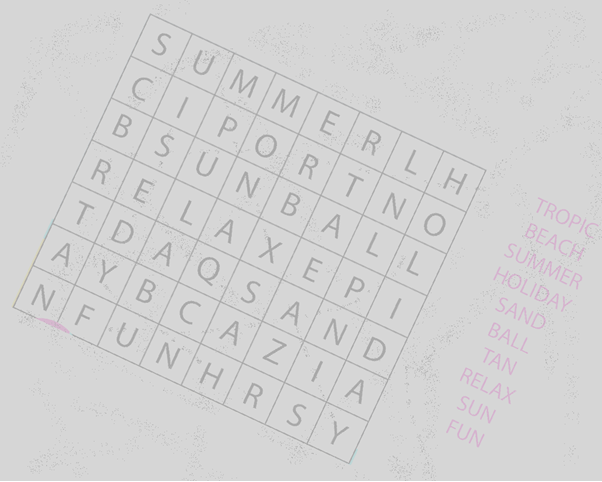
\includegraphics[width=300px,height=200px]{obrazky-figures/1.png}
\end{figure}

\subsection{Conversion en niveaux de gris (Grayscale)}

Nous utilisons la fonction grayscale, implémentée lors du premier TP de l'année. Cette fonction modifie chaque pixel de l'image selon la formule :

\[
\text{pixel} = 0.3r + 0.59g + 0.11b
\]

\begin{figure}[hbt]
	\centering
	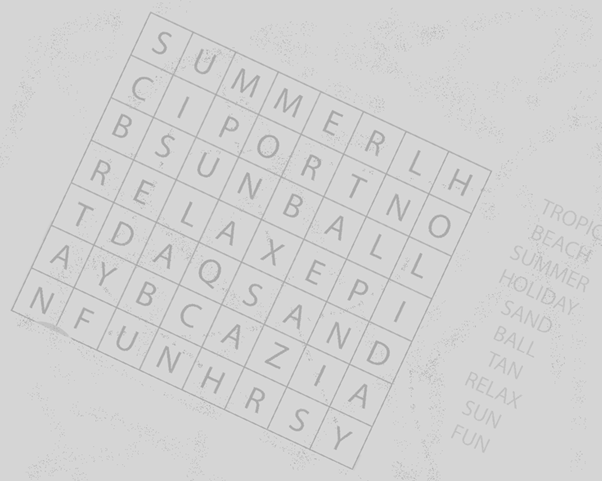
\includegraphics[width=300px,height=200px]{obrazky-figures/2.png}
\end{figure}

Cette opération transforme l'image en niveaux de gris.

\subsection{Filtre Médian}

Ce filtre parcourt chaque pixel de l'image. Pour chacun, il crée une liste contenant le pixel et ses 8 voisins adjacents. Le pixel est ensuite remplacé par la valeur médiane de cette liste (l'élément d'indice 4 une fois la liste triée). \\

\begin{figure}[hbt]
	\centering
	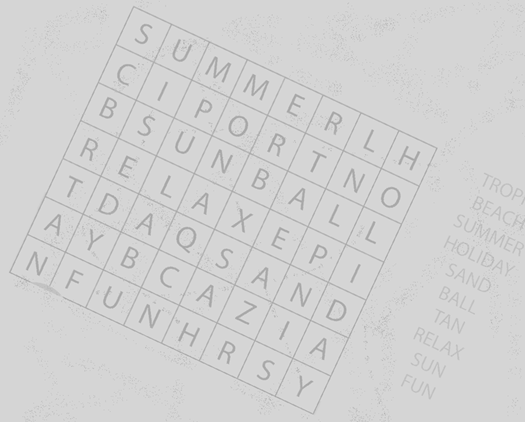
\includegraphics[width=300px,height=200px]{obrazky-figures/3.png}
\end{figure}

\subsection{Filtre Moyen}

Similaire au filtre médian, mais le pixel est remplacé par la moyenne des valeurs de la liste au lieu de la médiane. \\
Les filtres médian et moyen ont des effets subtils à l'œil nu, mais sont essentiels pour le bon fonctionnement des filtres suivants. \\

\begin{figure}[hbt]
	\centering
	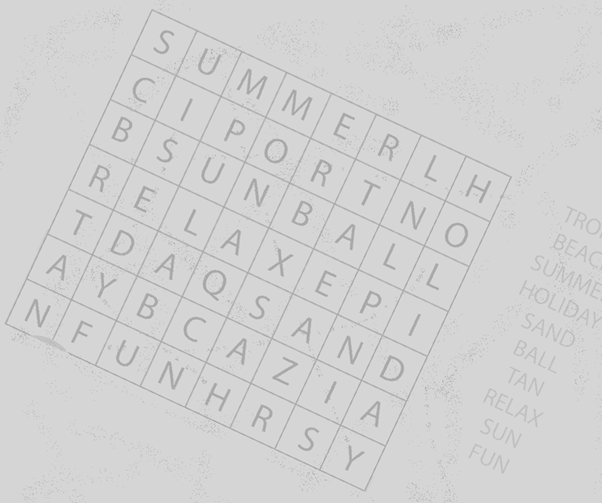
\includegraphics[width=300px,height=200px]{obrazky-figures/4.png}
\end{figure}

\subsection{Seuillage Adaptatif}

L'image est divisée en sous-parties, et un seuil est calculé pour chacune. Si la valeur d'un pixel est supérieure au seuil, il devient blanc ; sinon, il devient noir. La taille des sous-parties est déterminée par le niveau de bruit de l'image, calculé par la fonction "noiseLevel". \\\\
La fonction noiseLevel parcourt chaque pixel de l'image, calcule la moyenne du pixel et de ses voisins, puis applique la formule :

\[
valeur = 1 - \frac{pixel}{moyenne}
\]

\begin{figure}[hbt]
	\centering
	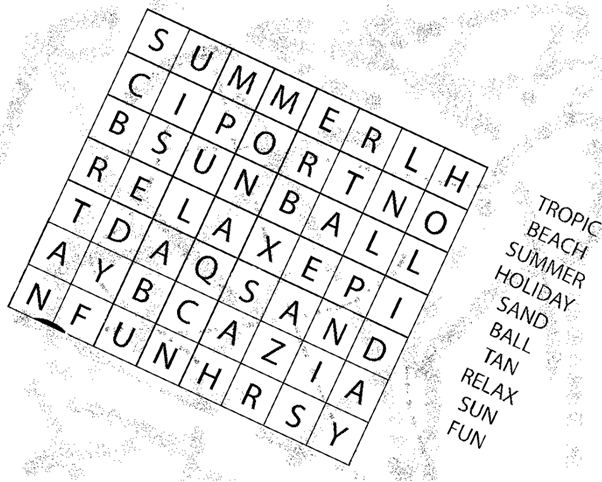
\includegraphics[width=300px,height=200px]{obrazky-figures/5.png}
\end{figure}

\noindent{Si cette valeur dépasse un seuil fixé à 0.5, le pixel est considéré comme du bruit.}

\subsubsection{Points d'amélioration :}

\begin{itemize}
  \item{Perfectionner les filtres existants}
  \item{Ajouter de nouveaux filtres (ex : filtre de Gauss, filtre de contraste)}
  \item{Optimiser les fonctions pour accélérer le processus}
\end{itemize}

\subsubsection{Difficultés rencontrées :}

\begin{itemize}
  \item{Documentation : trouver les méthodes les plus adaptées parmi les nombreuses options disponibles}
  \item{Erreurs de segmentation : identification difficile de l'origine du problème}
\end{itemize}

\subsubsection{Rotation d'image :}

La rotation d'image permet de positionner correctement la grille de mots croisés. Utilisant la bibliothèque SDL, nous chargeons l'image dans une texture, appliquons la rotation, puis transformons le résultat en surface pour le sauvegarder.

\chapter{Architecture et fonctions du solveur}

Le solveur est composé de 6 fonctions principales. Son objectif est de trouver un mot spécifique dans une grille de mots croisés stockée dans un fichier texte. Pour accomplir cette tâche, plusieurs paramètres sont pris en compte et traités par différentes fonctions.\\\\
Initialisation et structures de données :
\begin{itemize}
  \item{Des constantes sont définies pour la taille maximale de la grille, la longueur maximale d'un mot, et le nombre maximal de positions de départ possibles.}
  \item{Les variables globales sont initialisées, notamment "wordsearch", une matrice 2D représentant la grille de recherche.}
  \item{Une structure "position", est créée pour stocker les coordonnées x et y de chaque mot dans la grille.}
\end{itemize}

\lstdefinestyle{CStyle}{
    language=C,
    basicstyle=\ttfamily\small,
    keywordstyle=\color{blue}\bfseries,
    commentstyle=\color{green},
    stringstyle=\color{red},
    numbers=left,
    numberstyle=\tiny,
    numbersep=5pt,
    breaklines=true,
    showstringspaces=false,
    frame=single,
    tabsize=2
}

\begin{lstlisting}[style=CStyle]
#include <stdio.h>
#include <stdlib.h>
#include <string.h>
#include <ctype.h>

// Define constants for maximum sizes
#define MAX_GRID_SIZE 100   // Maximum size of the wordsearch grid
#define MAX_WORD_LENGTH 50  // Maximum length of a word to search
#define MAX_POSITIONS 1000  // Maximum number of starting positions for a word

// Structure to represent a position in the grid
typedef struct {
    int x;  // Row index
    int y;  // Column index
} Position;

// Global variables
char wordsearch[MAX_GRID_SIZE][MAX_GRID_SIZE];  // 2D array to store the wordsearch grid
int rows, cols;  // Dimensions of the wordsearch grid
\end{lstlisting}
\newpage
Fonctions principales :

\begin{enumerate}
  \item{is-valid-index : Cette fonction vérifie si une position donnée (line-num, col-num) est valide dans la grille.}
\end{enumerate}

\begin{lstlisting}[style=CStyle]
/**
 * Check if a given position is within the grid boundaries
 * line_num Row index
 * col_num Column index
 * return 1 if valid, 0 if not
 */
 
int is_valid_index(int line_num, int col_num) {
	return (line_num >= 0 && line_num < rows && col_num >= 0 && col_num < cols);
}
\end{lstlisting}

\begin{enumerate}[resume]
  \setcounter{enumi}{1}
  \item chars-match : Cette fonction vérifie si les caractères trouvés dans la grille correspondent au mot recherché.
\end{enumerate}

\begin{lstlisting}[style=CStyle]
/**
 * Check if the characters found match the beginning of the word
 * found Array of characters found in the grid
 * word Word being searched for
 * found_len Length of the found characters
 * return 1 if match, 0 if not
 */

int chars_match(const char* found, const char* word, int found_len) {
	for (int i = 0; i < found_len; i++) {
		if (found[i] != word[i]) {
			return 0;
		}
	}
	return 1;
}
\end{lstlisting}

\begin{enumerate}[resume]
  \setcounter{enumi}{2}
  \item print-coord : Affiche les coordonnées finales (première et dernière lettre) en fonction de la direction du mot trouvé.
\end{enumerate}

\begin{lstlisting}[style=CStyle]
/**
 * Print coordinates depending on the directions dx and dy
 * sx Start X
 * sy Start Y
 * ex End X
 * ey End Y
 * dx X direction (-1, 0, or 1)
 * dy Y direction (-1, 0, or 1)
 */
 
void print_coord(int sx, int sy, int ex, int ey, int dx, int dy) {
	if (dx == -1 && dy == 1) {
		printf("(%i,%i)(%i,%i)\n",ey,ex,sy,sx);
	}
	if (dx == 0 && dy == 1) {
		printf("(%i,%i)(%i,%i)\n",sy,sx,ey,ex);
	}
	if (dx == 1 && dy == 1) {
		printf("(%i,%i)(%i,%i)\n",sy,sx,ey,ex);
	}
	if (dx == -1 && dy == 0) {
		printf("(%i,%i)(%i,%i)\n",ey,ex,sy,sx);
	}
	if (dx == 1 && dy == 0) {
		printf("(%i,%i)(%i,%i)\n",sy,sx,ey,ex);
	}
	if (dx == -1 && dy == -1) {
		printf("(%i,%i)(%i,%i)\n",ey,ex,sy,sx);
	}
	if (dx == 0 && dy == -1) {
		printf("(%i,%i)(%i,%i)\n",ey,ex,sy,sx);
	}
	if (dx == 1 && dy == -1) {
		printf("(%i,%i)(%i,%i)\n",sy,sx,ey,ex);
	}
}
\end{lstlisting}

\begin{enumerate}[resume]
  \setcounter{enumi}{3}
  \item check-dir : Pour un mot donné, cette fonction vérifie s'il existe à partir d'un point de départ spécifié dans une direction donnée. Elle utilise :
    \begin{itemize}
      \item{Une liste "found-char" pour stocker les caractères rencontrés dans la direction (dx, dy).}
      \item{Une liste "final" pour enregistrer les coordonnées de chaque caractère trouvé. La fonction appelle ensuite print-coord pour afficher les résultats.}
    \end{itemize}
\end{enumerate}

\begin{lstlisting}[style=CStyle]
/**
 * Check if the word exists in a specific direction from a starting position
 * word Word to search for
 * start_pos Starting position
 * dx X direction (-1, 0, or 1)
 * dy Y direction (-1, 0, or 1)
 * return 1 if word found, 0 if not
 */
 
int check_dir(const char* word, Position start_pos, int dx, int dy) {
	char found_chars[MAX_WORD_LENGTH];
	Position current_pos = start_pos;
	Position positions[MAX_WORD_LENGTH];
	int pos_count = 0;
	int word_len = strlen(word);
	int final[2 * MAX_WORD_LENGTH];
	int index = 0;

	found_chars[0] = wordsearch[start_pos.x][start_pos.y];
	positions[pos_count] = start_pos;
	pos_count++;
	
	for (int i = 1; i < word_len; i++) {
		current_pos.x += dx;
		current_pos.y += dy;
		if (!is_valid_index(current_pos.x, current_pos.y)) {
			return 0;
		}

		found_chars[i] = wordsearch[current_pos.x][current_pos.y];
		positions[pos_count] = current_pos;
		pos_count++;

		if (!chars_match(found_chars, word, i + 1)) {
			return 0;
		}
	}

	// Word found, print the coordinates
	for (int x = 0; x < rows; x++) {
		for (int y = 0; y < cols; y++) {
			for (int z = 0; z < pos_count; z++) {
				if (positions[z].x == x && positions[z].y == y) {
					final[index] = x;
					index++;
					final[index] = y;
					index++;
				}
			}
		}
	}

	print_coord(final[0],final[1],final[index - 2],final[index - 1],dx,dy);
	return 1;
}
\end{lstlisting}

\begin{enumerate}[resume]
  \setcounter{enumi}{4}
  \item check-start : Appelle check-dir pour chaque direction possible à partir d'un point de départ. Retourne 1 si le mot est trouvé, 0 sinon.
\end{enumerate}

\begin{lstlisting}[style=CStyle]
/**
 * Check all 8 directions from a starting position for the word
 * word Word to search for
 * start_pos Starting position
 * return 1 if word found in any direction, 0 if not
 */
 
int check_start(const char* word, Position start_pos) {
	int directions[8][2] = {{-1,1}, {0,1}, {1,1}, {-1,0}, {1,0}, {-1,-1}, {0,-1}, {1,-1}};
	for (int i = 0; i < 8; i++) {
		if (check_dir(word, start_pos, directions[i][0], directions[i][1])) {
			return 1;
		}
	}
	return 0;
}
\end{lstlisting}

\begin{enumerate}[resume]
  \setcounter{enumi}{5}
  \item find-word : Fonction principale de recherche. Elle parcourt la grille pour trouver le premier caractère du mot, puis :
    \begin{itemize}
      \item{Attribue les coordonnées correspondantes à la structure "Position".}
      \item{Appelle check-start pour toutes les positions de départ potentielles.}
      \item{Affiche les coordonnées si le mot est trouvé, ou "Not found" dans le cas contraire.}
    \end{itemize}
\end{enumerate}

\begin{lstlisting}[style=CStyle]
/**
 * Find a word in the wordsearch grid
 * word Word to search for
 */
 
void find_word(const char* word) {
	Position start_pos[MAX_POSITIONS];
	int start_pos_count = 0;
	char first_char = word[0];

	// Find all positions of the first character of the word
	for (int i = 0; i < rows; i++) {
		for (int j = 0; j < cols; j++) {
			if (wordsearch[i][j] == first_char) {
				start_pos[start_pos_count].x = i;
				start_pos[start_pos_count].y = j;
				start_pos_count++;
			}
		}
	}

	// Check each starting position for the word
	for (int i = 0; i < start_pos_count; i++) {
		if (check_start(word, start_pos[i])) {
			return;
		}
	}
	printf("Not found\n");
}
\end{lstlisting}

\begin{enumerate}[resume]
  \setcounter{enumi}{5}
  \item La fonction principale du solveur :
    \begin{itemize}
      \item{Ouvre le fichier contenant la grille (en mode lecture).}
      \item{Convertit tous les caractères (du fichier et du mot recherché) en majuscules pour éviter les problèmes de casse.}
      \item{Appelle find-word pour effectuer la recherche.}
    \end{itemize}
\end{enumerate}

\begin{lstlisting}[style=CStyle]
int main(int argc, char* argv[]) {

	if (argc != 3) {
		printf("USAGE : ./solver FILE WORD\n");
		return 0;
	}
	char *filename;
	char *word;
	char line[MAX_GRID_SIZE];
	// Get the filename from the user
	filename = argv[1];
	// Open and read the file
	FILE *file = fopen(filename, "r");
	if (file == NULL) {
		printf("Unable to open file.\n");
		return 1;
	}

	// Read the wordsearch grid from the file
	rows = 0;
	while (fgets(line, sizeof(line), file) && rows < MAX_GRID_SIZE) {
		cols = strlen(line) - 1;  // -1 to remove newline
		for (int i = 0; i < cols; i++) {
			wordsearch[rows][i] = toupper(line[i]);
		}
		rows++;
	}

	fclose(file);

	// Get the word to search
	word = argv[2];

	// Convert word to uppercase for case-insensitive search
	for (int i = 0; word[i]; i++) {
		word[i] = toupper(word[i]);
	}

	find_word(word);
	return 0;
}
\end{lstlisting}

\chapter{Méthodes de détection et extraction d'éléments}

\subsection{I. Détection}

Le mode verbose (-v) a été intégré dès le début, facilitant le débogage en fournissant des informations détaillées sur les opérations effectuées. Cette fonctionnalité s'est avérée particulièrement utile dans cette partie complexe.\\\\
La détection des éléments d'intérêt dans l'image de mots mêlés se déroule en plusieurs étapes, utilisant principalement le filtre de Canny et la transformation de Hough.

\subsection{Détection des bords}

Pour la détection des bords de l'image, nous avons opté pour le filtre de Canny, qui offre une identification précise des contours avec une complexité raisonnable. Ce filtre comprend plusieurs étapes :

\subsection{Création automatisée d'un masque gaussien}

Une fonction génère un masque gaussien normalisé de taille et de force (écart-type $\sigma$) ajustables, offrant une flexibilité dans le code. Chaque terme du masque est calculé selon la formule :

\[
G(x,y) = \frac{1}{2\pi\sigma^2} \cdot e^{-\frac{x^2+y^2}{2\sigma^2}}
\]

\subsection{Application du filtre associé au masque gaussien}

La convolution est appliquée à tous les pixels de l'image. Pour chaque pixel $I(x,y)$, la convolution avec le masque gaussien G est effectuée :\\

\[
I'(x,y) = \sum_{m=-k}^k \sum_{n=-k}^n G(m,n) \cdot I(x+m,y+n)
\]

\noindent{Cette étape réduit le bruit et prépare l'image pour les étapes suivantes.}

\subsection{Calcul des gradients d'intensité et des orientations des contours}

Pour ce faire, nous commençons par créer un gradient $G_x$ et un gradient $G_y$ à l'aide d'un filtre de Sobel. Nous utilisons un masque 5x5 pour une précision accrue par rapport au masque 3x3 habituellement utilisé.\\

Sobel 3x3 :

\[G_x = \begin{bmatrix} -1 & 0 & 1 \\ -2 & 0 & 2 \\ -1 & 0 & 1 \end{bmatrix} * \text{Image}\]

\[G_y = \begin{bmatrix} 1 & 2 & 1 \\ 0 & 0 & 0 \\ -1 & -2 & -1 \end{bmatrix} * \text{Image}\]

Sobel 5x5 :

\[G_x = \begin{bmatrix} 
-2 & -1 & 0 & 1 & 2 \\
-4 & -2 & 0 & 2 & 4 \\
-6 & -3 & 0 & 3 & 6 \\
-4 & -2 & 0 & 2 & 4 \\
-2 & -1 & 0 & 1 & 2
\end{bmatrix} * \text{Image}\]

\[G_y = \begin{bmatrix}
2 & 4 & 6 & 4 & 2 \\
1 & 2 & 3 & 2 & 1 \\
0 & 0 & 0 & 0 & 0 \\
-1 & -2 & -3 & -2 & -1 \\
-2 & -4 & -6 & -4 & -2
\end{bmatrix} * \text{Image}\]

\noindent{La magnitude du gradient est calculée par :}
\[
G = \sqrt{(G_x)^2 + (G_y)^2}
\]
L'orientation des contours est déterminée par :
\[
\text{atan2}(G_x, G_y)
\]
arrondie à l'angle le plus proche parmi $\{$0°, 45°, 90°, 135°$\}$.

\subsection{Suppression des non-maxima}

Cette étape élimine les pixels ne correspondant pas à des bords réels en ne conservant que ceux ayant une magnitude de gradient maximale dans leur direction.

\subsection{Seuils de contours}

Deux seuils (élevé et faible) sont appliqués pour classer les pixels comme bords. Les pixels entre les deux seuils ne sont conservés que s'ils sont connectés à des bords forts.

\subsection{Sauvegarde de l'image obtenue}

L'image résultante après l'application du filtre Canny est sauvegardée pour être utilisée lors de la transformation de Hough.

\begin{figure}[hbt]
	\centering
	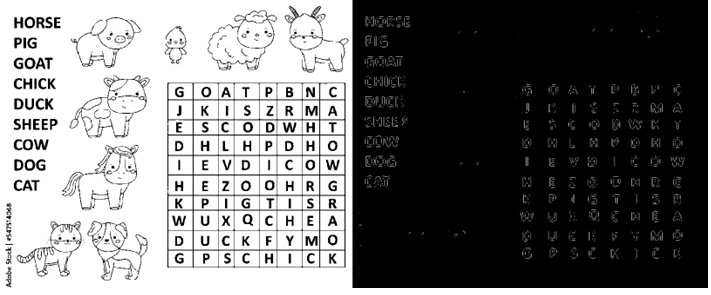
\includegraphics[width=420px,height=200px]{obrazky-figures/6.png}
\end{figure}

\subsection{Détection des lignes}

La transformation de Hough est utilisée pour identifier les lignes présentes dans l'image après la détection des bords. Elle transforme les points de l'espace image en une représentation paramétrique :
\[
\rho = x \cdot \cos(\theta) + y \cdot \sin(\theta)
\]
où $\rho$ est la distance à l'origine, et $\theta$ est l'angle de la ligne.
Malheureusement, la transformation de Hough n'est pas encore entièrement fonctionnelle dans notre implémentation.

\begin{figure}[hbt]
	\centering
	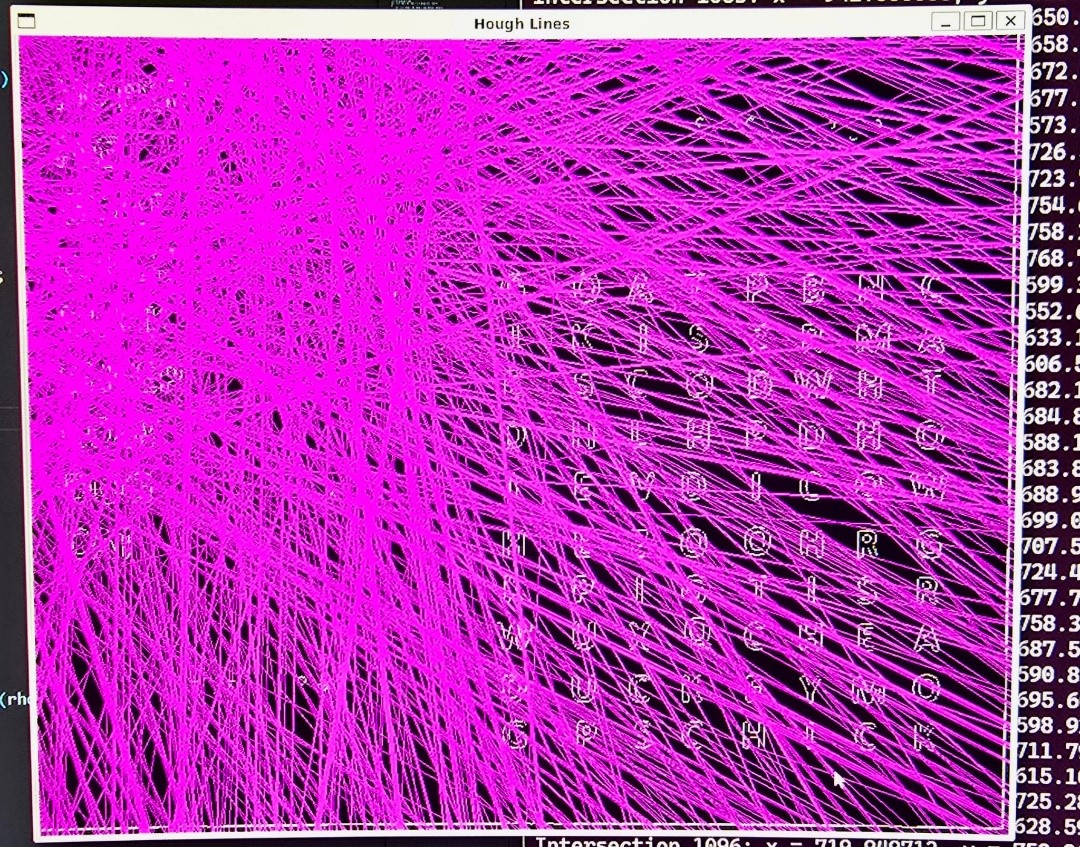
\includegraphics[width=300px,height=200px]{obrazky-figures/7.jpeg}
\end{figure}

\noindent{Après la détection des lignes, nous déterminons les coordonnées de la grille et de la liste de mots en identifiant les intersections des lignes détectées. Cela permet de localiser les cellules de la grille et d'en extraire les lettres qui la composent, ainsi que d'identifier la liste de mots pour en extraire les mots et les lettres correspondantes. Ces coordonnées seront ensuite utilisées pour découper la grille et sauvegarder les différents éléments.}\\

\noindent{Cependant, comme nous n'avons pas réussi à implémenter la transformation de Hough, cette partie n'a pas pu être réalisée. Néanmoins, nous avons trouvé une autre méthode pour obtenir les coordonnées de la grille et des lettres qui la composent. Voici les étapes de cette méthode :}

\begin{enumerate}
    \item \noindent Calcul du barycentre de l'image obtenue après l'application du filtre de Canny : 
    \begin{itemize}
        \item \noindent Le barycentre se situe sur la grille, car sa taille et son nombre de pixels influencent fortement l'image.
        \item \noindent Le barycentre est calculé de manière similaire à son utilisation en physique.
    \end{itemize}

    \item \noindent Itération en spirale autour du barycentre, en ignorant les points isolés jusqu'à atteindre un pixel blanc :
    \begin{itemize}
        \item \noindent Ce pixel sera nécessairement une lettre, puisque le barycentre est à l'intérieur de l'image et que les lignes de la grille ont été effacées par le filtre de Canny.
    \end{itemize}

    \item \noindent Récupération de la boîte englobante minimale (bounding box) pour cette lettre à partir du pixel obtenu et de l'image avant l'application du filtre de Canny.

    \item \noindent Ajustement de cette bounding box afin qu'elle soit carrée (en prenant la taille du plus grand côté) tout en restant centrée.
    \begin{itemize}
        \item \noindent On l'agrandit légèrement pour s'assurer qu'elle contient bien la lettre dans l'image après application du filtre de Canny.
    \end{itemize}

    \item \noindent Déplacement de cette bounding box depuis la première lettre trouvée dans les quatre directions (haut, bas, gauche et droite) sur l'image après application du filtre de Canny. En se décalant progressivement d'une taille de lettre, nous continuons jusqu'à ce que la densité de la bounding box cesse d'augmenter ou dépasse un certain seuil. Si aucune lettre n'est trouvée dans une direction après 2,5 fois la taille de la lettre, cela indique que nous avons atteint un bord de la grille.

    \item \noindent Détermination des quatre extrémités :
    \begin{itemize}
        \item \noindent Une fois ces coordonnées obtenues, elles permettent de définir la bounding box de la grille.
    \end{itemize}

    \item \noindent Calcul des positions des lettres dans la grille :
    \begin{itemize}
        \item \noindent Grâce à la bounding box ainsi qu'au nombre total de lettres dans la grille obtenues lors de la recherche des extrémités $((nb\_haut + nb\_bas + 1) * (nb\_gauche + nb\_droite + 1))$, nous déterminons les positions des lettres dans la grille.
    \end{itemize}
\end{enumerate}

\noindent{Bien que cette méthode semble complexe en raison du grand nombre d'étapes impliquées, elle n'est pas particulièrement gourmande en ressources informatiques.}

\subsection{Détermination des coordonnées des différents éléments}

Après la détection des lignes, nous déterminons les coordonnées de la grille et de la liste de mots en identifiant les intersections des lignes détectées. Cela permet de localiser les cellules de la grille et d'extraire les lettres, ainsi que de localiser la liste de mots.

\subsection{II. Découpage}

Le mode verbose (-v) est particulièrement utile pour vérifier la détection correcte de toutes les parties.\\\\
Le découpage de l'image suit les étapes suivantes :

\begin{enumerate}
  \item{Récupération des listes de coordonnées de la grille, de la liste de mots, des mots individuels, et des lettres.}
  \item{Récupération de la zone correspondante à l'aide de la bibliothèque SDL.}
  \item{Sauvegarde au format .bmp dans un dossier "result".}
\end{enumerate}

\noindent{Les fichiers sauvegardés suivent une convention de nommage claire : }

\begin{itemize}
  \item grid.bmp : image de la grille
\begin{figure}[hbt]
	\centering
	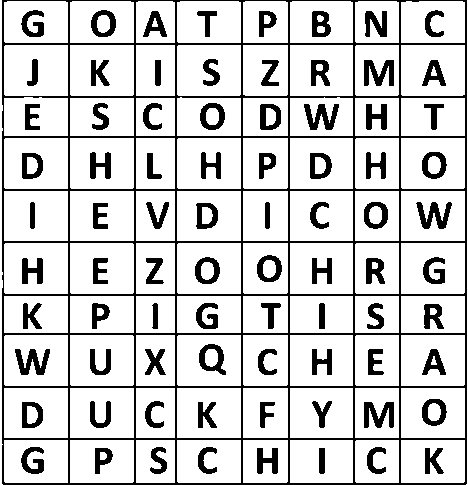
\includegraphics[width=200px,height=200px]{obrazky-figures/7.png}
\end{figure}
\newpage
  \item letterGrid\_1.bmp, letterGrid\_2.bmp, etc. : lettres de la grille
\begin{figure}[hbt]
	\centering
	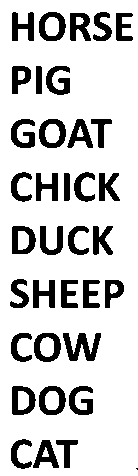
\includegraphics[width=100px,height=250px]{obrazky-figures/8.png}
\end{figure}
  \item words.bmp : liste des mots
\begin{figure}[hbt]
	\centering
	
\includegraphics[width=100px,height=100px]{obrazky-figures/9.png}
\end{figure}
  \item word\_1.bmp, word\_2.bmp, etc. : mots individuels
\begin{figure}[hbt]
	\centering
	
\includegraphics[width=200px,height=100px]{obrazky-figures/10.png}
\end{figure}
  \item letterWord1\_1.bmp, letterWord1\_2.bmp, etc. : lettres de chaque mot
\end{itemize}

Cette organisation facilite la récupération ultérieure par le réseau neuronal.
  \fi
  
  % Kompilace po částech (viz výše, nutno odkomentovat a zakomentovat input výše)
  % Compilation piecewise (see above, it is necessary to uncomment it and comment out input above)
  %\subfile{chapters/projekt-01-uvod-introduction}
  % ...
  %\subfile{chapters/projekt-05-zaver-conclusion}

  % Pouzita literatura / Bibliography
  % ----------------------------------------------
\ifslovak
  \makeatletter
  \def\@openbib@code{\addcontentsline{toc}{chapter}{Literatúra}}
  \makeatother
  \bibliographystyle{bib-styles/Pysny/skplain}
\else
\fi

  % vynechani stranky v oboustrannem rezimu
  % Skip the page in the two-sided mode
  \iftwoside
    \cleardoublepage
  \fi

  % Prilohy / Appendices
  % ---------------------------------------------
  \appendix
\ifczech
  \renewcommand{\appendixpagename}{Přílohy}
  \renewcommand{\appendixtocname}{Přílohy}
  \renewcommand{\appendixname}{Příloha}
\fi
\ifslovak
  \renewcommand{\appendixpagename}{Prílohy}
  \renewcommand{\appendixtocname}{Prílohy}
  \renewcommand{\appendixname}{Príloha}
\fi
%  \appendixpage

% vynechani stranky v oboustrannem rezimu
% Skip the page in the two-sided mode
%\iftwoside
%  \cleardoublepage
%\fi
  
\ifslovak
%  \section*{Zoznam príloh}
%  \addcontentsline{toc}{section}{Zoznam príloh}
\else
  \ifczech
%    \section*{Seznam příloh}
%    \addcontentsline{toc}{section}{Seznam příloh}
  \else
%    \section*{List of Appendices}
%    \addcontentsline{toc}{section}{List of Appendices}
  \fi
\fi
  \startcontents[chapters]
  \setlength{\parskip}{0pt} 
  % seznam příloh / list of appendices
  % \printcontents[chapters]{l}{0}{\setcounter{tocdepth}{2}}
  
  \ifODSAZ
    \setlength{\parskip}{0.5\bigskipamount}
  \else
    \setlength{\parskip}{0pt}
  \fi
  
  % vynechani stranky v oboustrannem rezimu
  \iftwoside
    \cleardoublepage
  \fi
  
  % Přílohy / Appendices
  \ifenglish
    \input{projekt-30-prilohy-appendices-en}
  \else
    \begin{thebibliography}{9}

\bibitem{sdl2}
Simple DirectMedia Layer (SDL2).
\textit{Official SDL Website}.
\url{https://www.libsdl.org/}

\bibitem{canny}
Canny, J. (1986).
A Computational Approach to Edge Detection.
\textit{IEEE Transactions on Pattern Analysis and Machine Intelligence}, 
PAMI-8(6), 679-698.

\bibitem{hough}
Duda, R. O., & Hart, P. E. (1972).
Use of the Hough transformation to detect lines and curves in pictures.
\textit{Communications of the ACM}, 15(1), 11-15.

\bibitem{gaussian}
Shapiro, L. G. & Stockman, G. C. (2001).
Computer Vision.
Prentice Hall.

\bibitem{sobel}
Sobel, I., & Feldman, G. (1968).
A 3x3 Isotropic Gradient Operator for Image Processing.
\textit{Stanford Artificial Intelligence Project (SAIL)}.

\bibitem{adaptive_threshold}
Bradley, D., & Roth, G. (2007).
Adaptive Thresholding using the Integral Image.
\textit{Journal of Graphics Tools}, 12(2), 13-21.

\bibitem{ocr}
Mori, S., Nishida, H., & Yamada, H. (1999).
Optical Character Recognition.
John Wiley & Sons.

\bibitem{image_processing}
Gonzalez, R. C., & Woods, R. E. (2018).
Digital Image Processing (4th ed.).
Pearson.

\end{thebibliography}
  \fi
  
  % Kompilace po částech (viz výše, nutno odkomentovat)
  % Compilation piecewise (see above, it is necessary to uncomment it)
  %\subfile{projekt-30-prilohy-appendices}
  
\end{document}
